
%------------------------------------------------------------------------
%
%    Copyright (C) 1985-2020  Georg Umgiesser
%
%    This file is part of SHYFEM.
%
%    SHYFEM is free software: you can redistribute it and/or modify
%    it under the terms of the GNU General Public License as published by
%    the Free Software Foundation, either version 3 of the License, or
%    (at your option) any later version.
%
%    SHYFEM is distributed in the hope that it will be useful,
%    but WITHOUT ANY WARRANTY; without even the implied warranty of
%    MERCHANTABILITY or FITNESS FOR A PARTICULAR PURPOSE. See the
%    GNU General Public License for more details.
%
%    You should have received a copy of the GNU General Public License
%    along with SHYFEM. Please see the file COPYING in the main directory.
%    If not, see <http://www.gnu.org/licenses/>.
%
%    Contributions to this file can be found below in the revision log.
%
%------------------------------------------------------------------------

\shy{} is the System of HydrodYnamic Finite Element Modules that can be used to 
resolve the dynamics of the seas, coastal areas, lagoons, estuaries and lakes. 

It is an open source 3D hydrodynamic finite element model
which solves the primitive equations - vertically integrated over each layer -
considering tidal, atmospheric and density-driven forces. 
The model has been already applied 
to simulate hydrodynamics in the Mediterranean Sea \cite{ferrarin13:med,
Ferrarin2018_mmba}, in the Black Sea \cite{Bajo14:black}, in the Adriatic Sea 
\cite{bella10:3d,Ferrarin2016_mgsed,Ferrarin2017_adlag}, and in several coastal 
systems \cite{Umgiesser1410lags}.


SHYFEM uses a semi-implicit algorithm for integration in time, which combines the advantages of the explicit and the implicit schemes. The bottom friction is computed introducing the Strickler formulation, so that the friction coefficient is not a constant but varies with water depth. The state of the art turbulence closure model GOTM is used for simulating the sub-grid processes governing the variability on the vertical direction.

At the open boundaries the water levels are prescribed in accordance with the Dirichlet condition, while at the closed boundaries only the normal velocity is set to zero and the tangential velocity is a free parameter. This allows the transport variables to be solved explicitly without solving any linear system. Compared to a fully implicit solution of the shallow water equations solving a linear system for the water levels, it reduces the dimensions of the matrix to one third.

The hydrodynamic module is fully coupled with a state of the art wind wave model accounting for wave generation, propagation and dissipation processes in both coastal areas and open ocean. In particular a two-way coupling based on radiation stress theory  allows to reproduce both the effect of wind wave on water currents and water levels computation and vice versa.

The model also consists on an Eulerian and a Lagrangian transport module to simulate the advection and diffusion of active tracers into the waters. The two approaches allow to simulate both dissolved chemicals such as nutrients or heavy metals and dispersed tracers such as hydrocarbons giving the possibility to include a reactor to consider the time variation of the tracers masses.

The hydrodynamic model SHYFEM has been coupled and integrated with other numerical models:
\begin{itemize}
 \item   SEDTRANS sediment transport model
 \item   EUTRO-WASP ecological model
 \item  ERSEM-BFM ecosystem model
  \item  WWMII spectral wind wave model
  \item  GOTM turbulence closure model
\end{itemize}

Moreover, the model provides a tidal potential module and a non-hydrostatic module.
The scheme of \shy{} modular structure is shown in \Fig \ref{module}.


\begin{figure}[htbp]
\centering
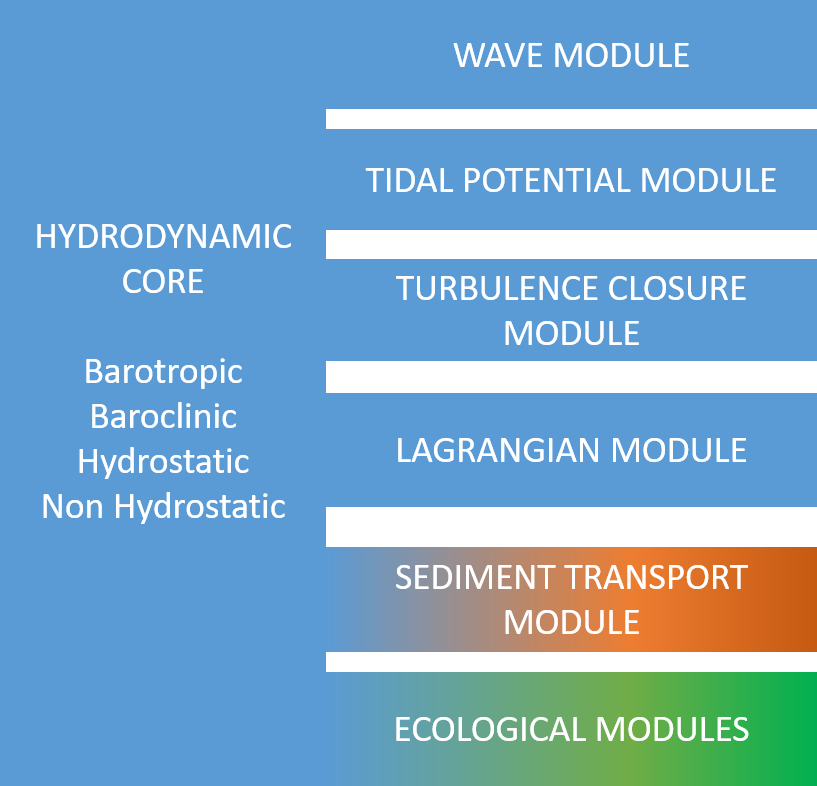
\includegraphics[scale=0.5]{module_scheme.png}
\caption{Model structure and available modules}
\label{module}
\end{figure}

The program uses finite elements for the resolution of
the hydrodynamic equations. These finite elements, together with an
effective semi-implicit time resolution algorithm, makes this program
especially suitable for applications in areas with a complicated geometry
and bathymetry (\Fig \ref{grids}).

\begin{figure}[htbp]
\centering
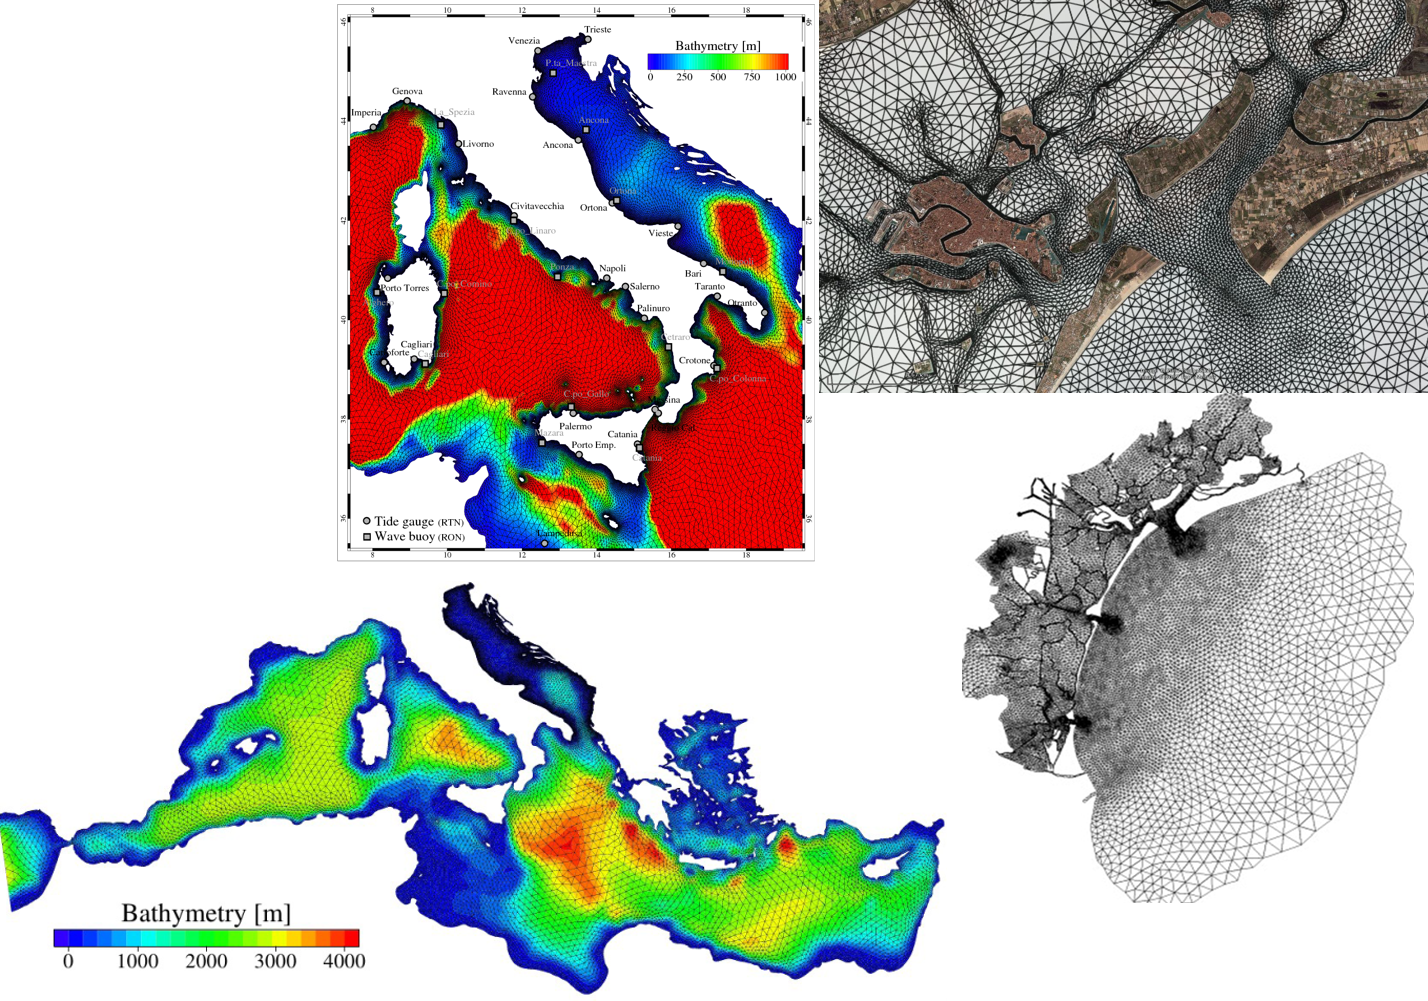
\includegraphics[scale=0.45]{overview_model.png}
\caption{Example modelled domains at different spatial scales, from the Mediterranean Sea to the channels of the Venice Lagoon.}
\label{grids}
\end{figure}


The program \shy{} resolves the depth integrated shallow water equations
and can use both two- or three-dimensional formulations, depending
on the user's needs.

The finite element method has
an advantage over other methods (e.g., finite differences) because it
well adapts to problems dealing with complex
bathymetries and geometries, allowing more flexibility with its subdivision of the system in triangles
varying in form and size.  This flexibility can be used also in situations
where it is not desired to have uniform resolution of the whole basin,
but where a focus in resolution is needed only in some parts of the area.

It is possible to simulate shallow water flats, i.e., tidal marshes
that in a tidal cycle may be underwater during high tide and
dry during ebb tide. This phenomenon is handled by the model
in a mass conserving way, as explained in appendix \ref{mass}.

Finite element methods have been introduced into hydrodynamics since 1973
and have been extensively applied to shallow water equations by numerous
authors \cite{Grotkop73, Taylor75, Herrling77, Herrling78, Holz82}.

% FIXME - new references

The model presented here \cite{Umgies86, Umgies93} uses the mathematical
formulation of the semi-implicit algorithm that decouples the solution
of the water levels and velocity components from each other leading to
smaller systems to solve. Models of this type have been presented from
1971 on by many authors \cite{Kwizak71, Duwe82, Backhaus83}.

